%! TEX program = xelatex
\documentclass[UTF8,a4paper,12pt,fontset=fandol]{ctexart}

\usepackage[top=2.5cm,bottom=2.5cm,left=2.5cm,right=2.5cm]{geometry}
\usepackage{amsmath,amssymb,bm}
\usepackage{booktabs,tabularx,multirow,longtable,array}
\usepackage{graphicx,float,subcaption}
\usepackage{enumitem}
\usepackage{xcolor}
\usepackage{listings}
\usepackage{url}
\usepackage[hidelinks]{hyperref}
\usepackage{appendix}

\graphicspath{{figures/}{figures/q2/}}
\setlength{\parindent}{2em}
\setlength{\parskip}{0pt}
\linespread{1.25}
\pagestyle{plain}

\ctexset{
  section={format=\zihao{4}\bfseries,beforeskip=1.2ex,afterskip=0.8ex},
  subsection={format=\zihao{-4}\bfseries,beforeskip=1ex,afterskip=0.6ex},
  subsubsection={format=\zihao{-4}\bfseries,beforeskip=0.8ex,afterskip=0.4ex}
}

\captionsetup{font=small,labelsep=quad}
\setlist{nosep,leftmargin=2em}

\lstset{
  basicstyle=\small\ttfamily,
  numbers=left,
  numberstyle=\tiny\color{gray},
  frame=single,
  breaklines=true,
  showstringspaces=false,
  keywordstyle=\color{blue!70!black},
  commentstyle=\color{green!45!black},
  stringstyle=\color{purple}
}

\begin{document}
\pagenumbering{arabic}
\setcounter{page}{1}

% ======================== 摘要专用页 ========================
\begin{center}
  {\zihao{3}\bfseries NIPT的时点选择与胎儿的异常判定}
\end{center}

\begin{center}
  {\zihao{4}\bfseries 摘\quad 要}
\end{center}

% 摘要应在四问结果完成后统一撰写，并给出关键数值结论。
本文针对NIPT检测时点选择与胎儿异常判定问题，基于男胎和女胎的纵向检测数据开展建模分析。当前已完成问题背景、问题要求、问题分析以及问题二的建模与结果整理，其余问题完成后再统一补充摘要中的方法、关键结果和模型评价。

\vspace{0.8em}
\noindent\textbf{关键词：}无创产前检测；Logistic回归；CART分组；敏感性分析

\newpage

% =========================== 正文 ===========================
\section{问题重述}

\subsection{问题背景}

无创产前检测（Non-invasive Prenatal Test，NIPT）是一种通过采集孕妇血液并分析其中胎儿游离DNA片段，对胎儿染色体异常风险进行评估的产前检测技术。与传统侵入性产前诊断方式相比，NIPT具有安全性较高、检测过程方便等特点，在唐氏综合征、爱德华氏综合征和帕陶氏综合征等常见染色体异常的早期筛查中具有重要作用。

NIPT检测结果的可靠性受到孕周、孕妇身体质量指数以及测序质量等多种因素影响。对于男胎，当Y染色体浓度达到一定水平时，检测结果才具有较高的可信度。若检测时间过早，胎儿游离DNA浓度可能不足，从而增加检测失败或结果不稳定的可能；若检测时间过晚，又可能缩短发现异常后的临床处理时间。因此，如何在检测可靠性与早期发现风险之间取得平衡，是NIPT时点选择中的重要问题。

此外，不同孕妇在年龄、身高、体重、BMI和妊娠状况等方面存在个体差异，采用统一的检测时间难以适用于所有人群。对于不携带Y染色体的女胎，还需要结合染色体Z值、GC含量和读段质量等信息建立异常判定方法。基于上述背景，本文利用给定的男胎与女胎NIPT检测数据，研究男胎检测时点的合理选择，并建立女胎染色体异常判定模型。

\subsection{问题要求}

针对附件所给出的男胎与女胎NIPT检测数据，本文需要完成以下四项任务：

\textbf{问题一：}分析男胎Y染色体浓度与孕妇检测孕周、BMI及其他相关指标之间的关系，建立相应的关系模型，并检验模型及相关变量的显著性。

\textbf{问题二：}在BMI是影响男胎Y染色体浓度最早达标时间主要因素的条件下，对男胎孕妇进行合理的BMI分组，给出各组BMI区间和最佳NIPT检测时点，使潜在风险尽量降低，并分析检测误差的影响。

\textbf{问题三：}在问题二基础上，进一步考虑年龄、身高、体重等个体因素，以及检测误差和Y染色体浓度达标比例的影响，重新确定合理的BMI分组和各组最佳NIPT检测时点。

\textbf{问题四：}针对女胎不携带Y染色体的特点，以附件AB列中的13、18、21号染色体非整倍体结果作为异常判定依据，综合考虑染色体Z值、GC含量、测序读段指标、相关比例、X染色体浓度和BMI等因素，建立女胎异常判定方法。

\section{问题分析}

\subsection{问题一分析}

问题一研究男胎Y染色体浓度与检测孕周、BMI及其他指标之间的数量关系，是后续确定最佳检测时点的基础。首先统一孕周表示方式并进行描述性统计和可视化，再建立Y染色体浓度与各影响因素之间的关系模型，通过参数显著性、拟合优度和残差分析评价模型。由于同一孕妇可能存在多次检测记录，还需处理个体内相关性，预期得到孕周、BMI等因素的影响方向、影响程度及统计显著性。

\subsection{问题二分析}

问题二承接问题一，将研究目标由“解释Y染色体浓度的变化”转化为“确定不同BMI人群的最佳NIPT检测时点”。利用问题一中孕周、BMI与Y染色体浓度之间的关系，将Y染色体浓度达到或超过$4\%$定义为达标，估计不同BMI和孕周下的达标概率。在此基础上对BMI进行数据驱动分组，并在检测可靠性与延迟发现风险之间进行权衡，为每组选择尽可能早且可靠的检测时点。最后通过重复测序、Bootstrap和误差扰动分析结论的稳定性。

\subsection{问题三分析}

问题三是对问题二的扩展。问题二主要依据BMI进行群体分组，但实际达标时间还可能受到年龄、身高、体重、妊娠方式和测序质量的影响。因此需在保留BMI分组这一实际应用形式的同时，建立多因素达标概率模型，将更多个体特征纳入组内风险计算，重新确定各组最佳检测时点，并检验误差条件下分组边界和推荐时点的稳定性。

\subsection{问题四分析}

问题四的研究对象由男胎转为女胎。本文将附件AB列为空定义为无异常，出现T13、T18、T21或其组合定义为异常；以各染色体Z值、X染色体浓度、GC含量、测序读段指标、BMI和孕周等作为候选特征建立分类模型。训练集和测试集按孕妇代码划分，避免重复记录造成信息泄漏，并使用召回率、特异度、F1值和ROC--AUC等指标评价女胎异常判定效果。

\section{模型假设}

\begin{enumerate}
  \item 假设附件中的检测记录及字段含义真实可靠，清洗过程中仅对同次采血的重复测序进行合并，不改变原始生物学观测。
  \item 假设同次采血的Y染色体浓度测量误差相互独立、均值为零，且其方差在研究范围内近似稳定，以便利用重复测序差异估计测量误差。
  \item 假设在$10$至$25$孕周的研究区间内，同一BMI水平下的群体达标概率不会随孕周增加而下降；观测中的局部波动主要由测量误差和个体差异造成。
  \item 问题二以首次检测时BMI作为基线BMI，并假设其能够代表孕妇所属的BMI群体，避免使用达标后的BMI造成时间信息倒置。
  \item 假设样本所代表地区的检测流程在研究期内保持一致，模型结论主要用于相似高BMI人群的群体时点建议，不直接替代个体临床诊断。
\end{enumerate}

\section{数据预处理}

\subsection{重复检测记录的合并}

男胎原始工作表包含1082条检测记录和267名孕妇。数据中既有同一孕妇的多次抽血，也有同次采血的重复测序。为避免将技术重复误认为独立生物样本，本文以“孕妇代码、检测日期、检测抽血次数”为联合键合并同次采血记录，对Y染色体浓度取中位数，并保留最小值、最大值、极差及是否跨越$4\%$阈值等信息。共识别19组同次采血重复测序，合并后得到1063次独立采血记录。

\begin{table}[H]
  \centering
  \caption{问题二数据清洗统计}
  \label{tab:q2-clean-summary}
  \begin{tabular}{cc}
    \toprule
    项目 & 数量 \\
    \midrule
    原始检测记录 & 1082条 \\
    男胎孕妇 & 267人 \\
    清洗后独立采血记录 & 1063次 \\
    同次采血重复测序组 & 19组 \\
    重复测序跨越$4\%$阈值 & 4组 \\
    \bottomrule
  \end{tabular}
\end{table}

\subsection{变量标准化与达标状态构造}

将“$a\mathrm{w}+b$”形式的孕周转换为连续周数：

\begin{equation}
  W=a+\frac{b}{7}.
  \label{eq:week-convert}
\end{equation}

利用体重除以身高平方复核BMI，差异均小于0.02。为避免把达标之后发生的体重变化反向用于预测，问题二采用每名孕妇首次检测时的BMI作为基线BMI。定义第$i$名孕妇第$j$次独立采血的达标状态为

\begin{equation}
  D_{ij}=\mathbb{I}\!\left(Y_{ij}\geq 0.04\right),
  \label{eq:q2-status}
\end{equation}

其中$Y_{ij}$表示Y染色体浓度。GC含量略低于$40\%$的记录仅设置质量标记而不机械删除，避免一次性剔除大量临界样本。

\subsection{删失结构说明}

267名孕妇中，217人在第一次检测时已经达标，只能确定真实达标时间早于首次检测，属于左删失；43人的真实达标时刻位于相邻两次检测之间，属于区间删失；7人在最后一次检测时仍未达标，属于右删失。因此，首次观测到达标的孕周不能直接等同于精确的生理达标时间，后续模型应尽量使用全部纵向检测记录。

% 问题一由负责同学完成后，将正文写入本文件。
% 建议结构：变量与相关性分析、关系模型、显著性检验、结果解释。

\section{问题二的模型建立与求解}

\subsection{与问题一的联系及总体思路}

问题一用于识别孕周、BMI等指标与Y染色体浓度之间的关系；问题二进一步把这种关系转化为可执行的检测决策。其核心不再只是解释Y染色体浓度如何变化，而是回答“不同BMI孕妇在何时检测，既能保证足够的达标概率，又能尽量避免延迟发现风险”。

为此，本文采用“纵向达标概率建模—可靠性约束下的时点反演—CART自动分组—误差与稳定性检验”的四步框架。首先利用全部1063次独立采血记录建立达标概率模型；随后反演不同BMI水平达到目标可靠性的最早孕周；再利用一维CART将连续BMI压缩为若干可解释区间；最后使用Bootstrap和重复测序误差扰动检验结果稳定性。

\subsection{首次观测达标孕周的探索性分析}

先对260名曾观测到Y染色体浓度达标的孕妇，绘制基线BMI与首次观测达标孕周$T$的散点图，结果见图~\ref{fig:q2-bmi-week}。Spearman秩相关系数为$\rho=0.0878$，双侧检验$p=0.158$，表明二者仅呈极弱且不显著的正相关。

\begin{figure}[H]
  \centering
  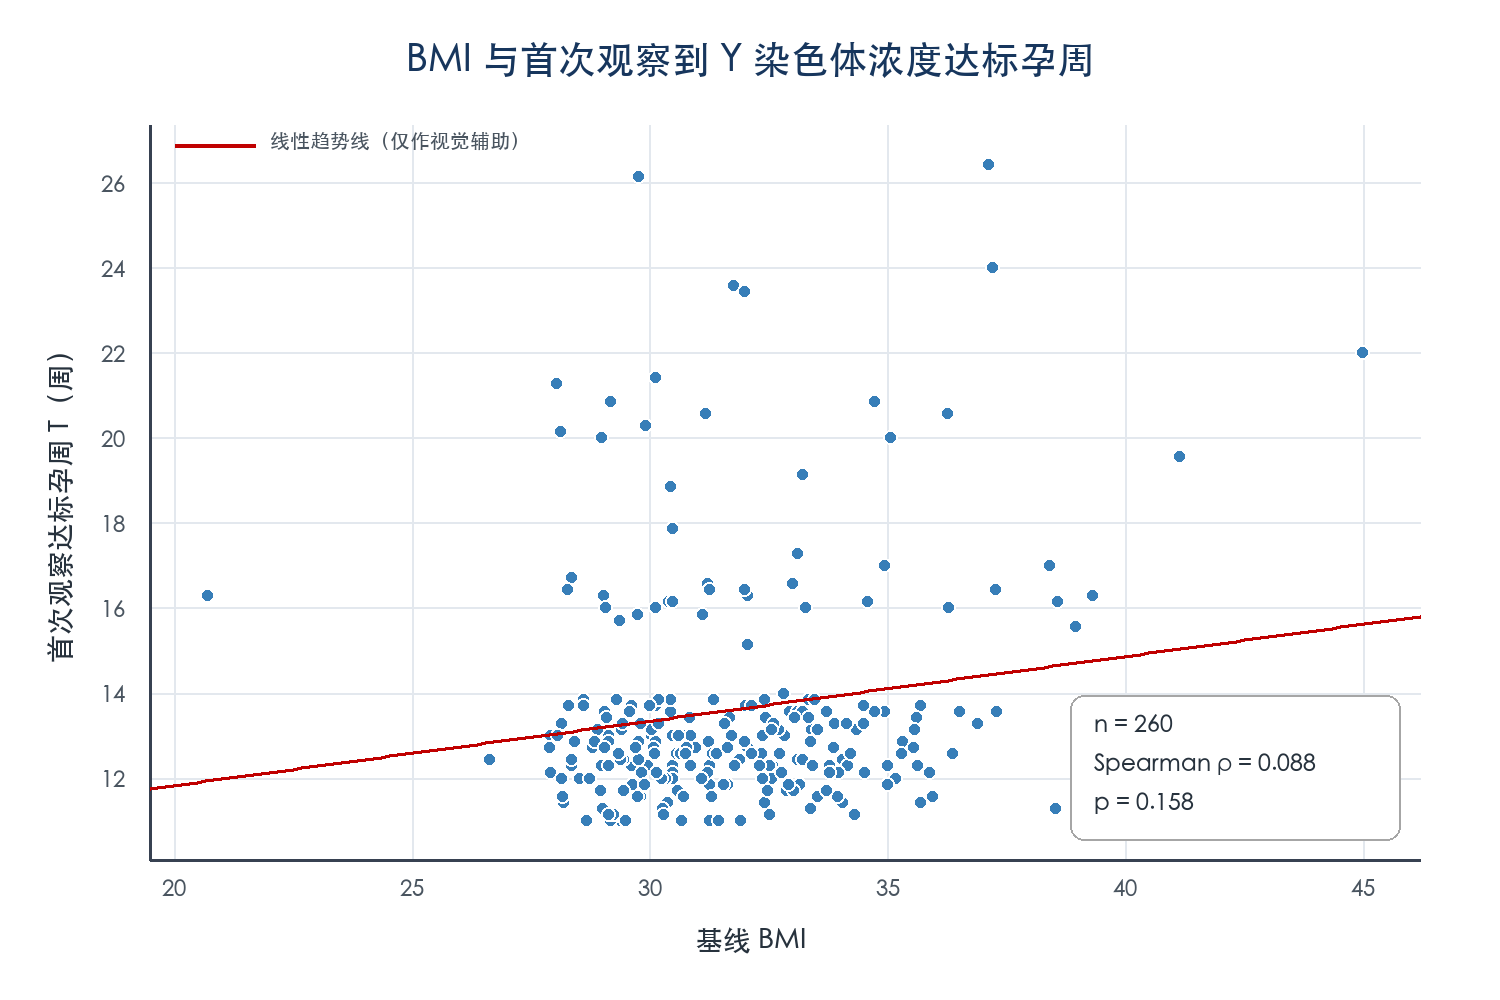
\includegraphics[width=0.92\textwidth]{q2_bmi_first_observed_week.png}
  \caption{基线BMI与首次观测Y染色体浓度达标孕周}
  \label{fig:q2-bmi-week}
\end{figure}

上述弱相关不能直接解释为BMI没有作用。由第~\ref{eq:q2-status}式可知，达标时间的观测依赖于实际采样安排；特别是首次检测已经达标的217名孕妇，其真实达标时刻只能确定为早于首次检测。若直接对首次观测达标孕周进行普通回归或CART分组，会把“何时接受检测”与“何时生理达标”混为一谈。因此，本文不把图~\ref{fig:q2-bmi-week}中的$T$作为主模型的连续响应变量，而改用每名孕妇的全部纵向检测记录建立达标概率模型。

\subsection{纵向达标概率模型}

\subsubsection{模型设定}

设$W_{ij}$为第$i$名孕妇第$j$次独立采血时的孕周，$B_i$为其基线BMI，$D_{ij}$为第~\ref{eq:q2-status}式定义的达标状态。记

\begin{equation}
  p_{ij}=P\!\left(D_{ij}=1\mid W_{ij},B_i\right).
  \label{eq:q2-probability}
\end{equation}

候选模型包括线性Logistic回归、含二次项与交互项的Logistic回归、样条Logistic回归和梯度提升树，并设置仅使用总体达标率的常数模型作为基准。线性Logistic模型写为

\begin{equation}
  \operatorname{logit}(p_{ij})
  =\beta_0+\beta_1W_{ij}+\beta_2B_i.
  \label{eq:q2-logistic}
\end{equation}

由于各孕妇的检测次数不同，若给每条记录相同权重，检测次数较多的孕妇会对参数估计产生过大影响。因此，将第$i$名孕妇全部记录的总权重设为1，每条记录权重取其检测次数的倒数。

\subsubsection{分组交叉验证与模型选择}

为防止同一孕妇的多次记录同时出现在训练集和验证集中，采用以孕妇代码为分组单位的五折交叉验证。模型选择以LogLoss为主要指标，Brier得分和AUC为辅助指标；LogLoss和Brier越小，说明概率预测越准确，AUC越大，说明区分达标与未达标记录的能力越强。相关方法可参考Logistic回归与统计学习理论\cite{hosmer2013applied,hastie2009elements}。

\begin{table}[H]
  \centering
  \caption{候选达标概率模型的分组五折交叉验证结果}
  \label{tab:q2-model-cv}
  \begin{tabular}{ccccc}
    \toprule
    模型 & LogLoss & 标准误 & Brier & AUC \\
    \midrule
    二次交互Logistic & 0.3853 & 0.0273 & 0.1127 & 0.5798 \\
    线性Logistic & 0.3866 & 0.0273 & 0.1130 & 0.5804 \\
    基准常数模型 & 0.3912 & 0.0242 & 0.1147 & 0.5000 \\
    样条Logistic & 0.3920 & 0.0320 & 0.1144 & 0.5705 \\
    梯度提升树 & 0.3992 & 0.0349 & 0.1156 & 0.6061 \\
    \bottomrule
  \end{tabular}
\end{table}

\begin{figure}[H]
  \centering
  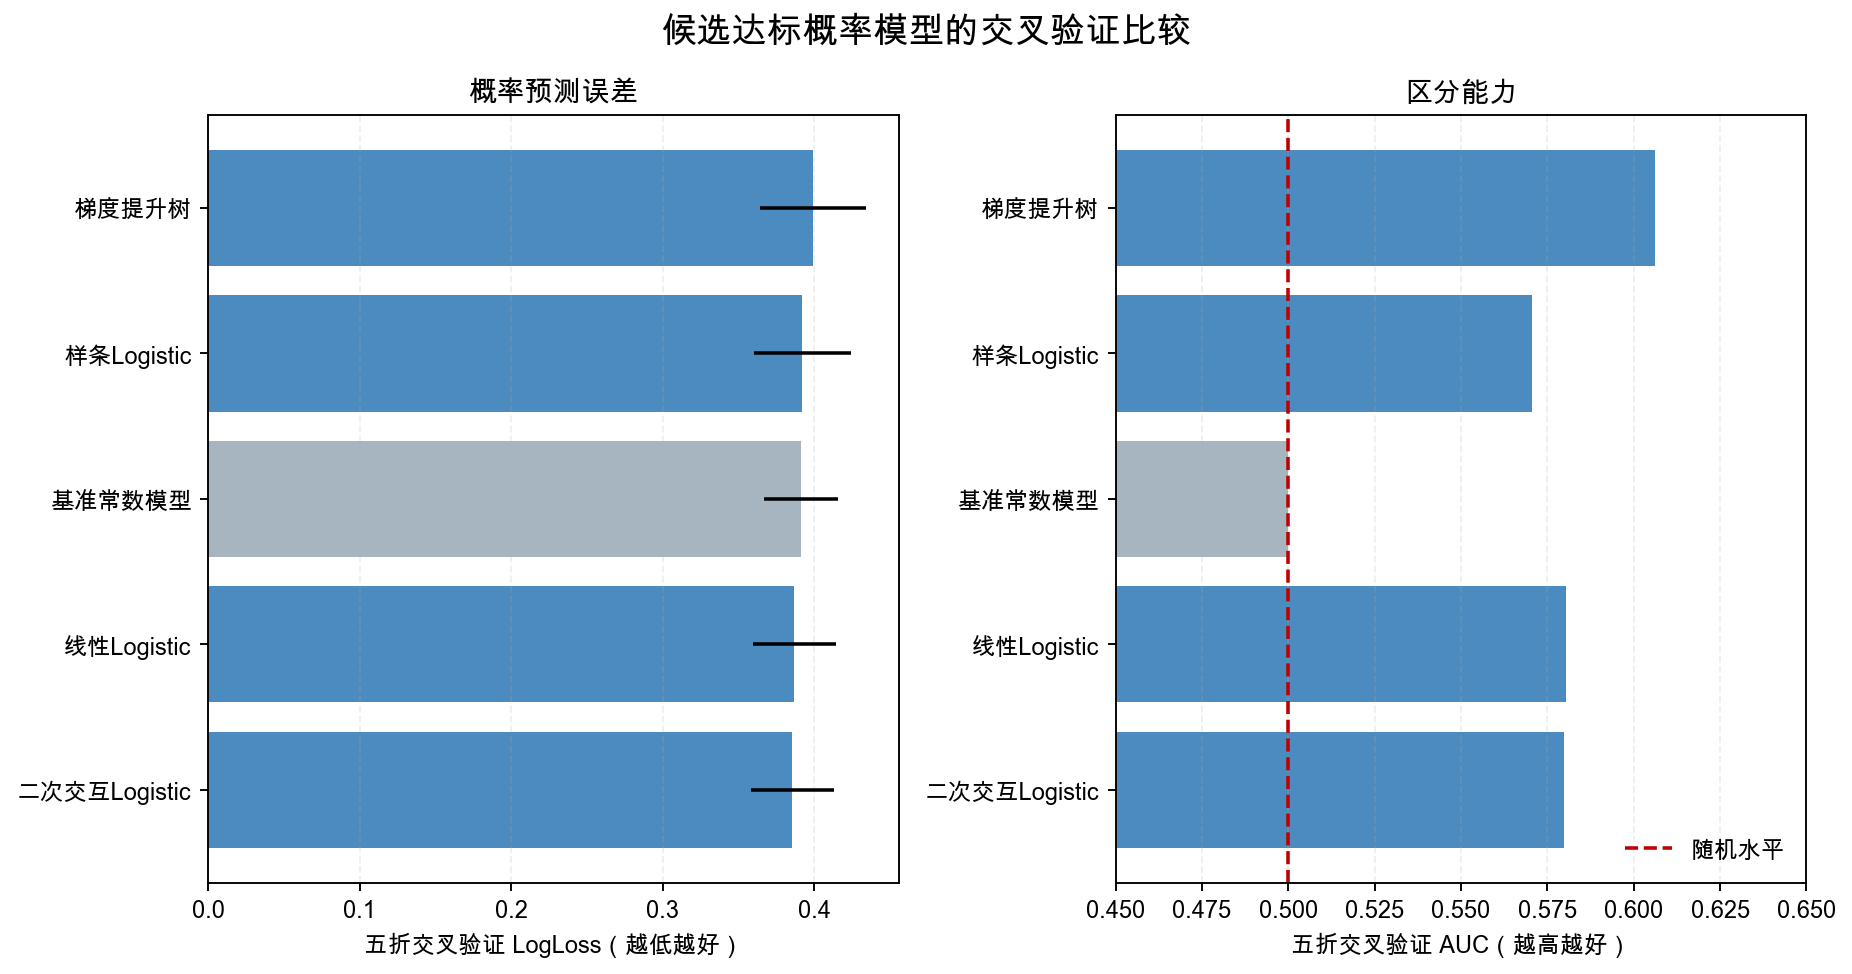
\includegraphics[width=0.96\textwidth]{q2_model_comparison.png}
  \caption{候选达标概率模型的交叉验证比较}
  \label{fig:q2-model-comparison}
\end{figure}

由表~\ref{tab:q2-model-cv}和图~\ref{fig:q2-model-comparison}可见，二次交互Logistic取得最低LogLoss，但其与线性Logistic的差值仅为0.0013，远小于相应交叉验证标准误0.0273。依据一标准误差规则，在预测误差没有显著恶化的情况下优先选择结构更简单的线性Logistic模型。梯度提升树虽然AUC相对较高，但LogLoss和Brier均较差，说明其概率校准能力不足，不适合作为本题时点反演的主模型。

将线性Logistic模型系数换算回原始量纲，得到

\begin{equation}
  \operatorname{logit}(p)
  =5.3712+0.0412W-0.1285B.
  \label{eq:q2-final-logistic}
\end{equation}

孕周系数为正、BMI系数为负，表示在控制另一变量后，孕周增加有利于Y染色体浓度达标，而BMI升高会降低同一孕周下的达标概率。不过，最终模型AUC仅为0.5804，说明只使用BMI和孕周时个体区分能力有限。因此，本文将该模型用于群体检测时点决策，不将其解释为高精度个体诊断模型。

\subsection{可靠性约束下的最佳检测时点}

题目要求同时兼顾检测准确性和尽早发现风险。本文采用词典序决策准则：首先满足预设的达标可靠性，在满足可靠性的可行孕周中选择最早时点。为符合群体达标概率一般不随孕周下降的规律，对预测概率曲线施加累积最大值约束。定义给定BMI下达到$90\%$预测达标概率的最早孕周为

\begin{equation}
  t_{0.90}(B)
  =\min\left\{w:P(Y\geq0.04\mid B,w)\geq0.90\right\},
  \quad 10\leq w\leq25.
  \label{eq:q2-target-week}
\end{equation}

对第$g$个BMI组，令$\bar p_g(w)$为组内孕妇在孕周$w$的平均预测达标概率，则推荐时点为

\begin{equation}
  t_g^{*}=\min\left\{w:\bar p_g(w)\geq q_g\right\}.
  \label{eq:q2-group-week}
\end{equation}

通常取$q_g=0.90$。若某组在25周内仍不能达到$90\%$，则将可行阈值降为$85\%$，在达到该阈值的最早孕周先行检测，并对未达标样本安排复测。该规则避免为了追求小幅准确率提升而把检测过度推迟至治疗窗口更加紧张的阶段。

\subsection{基于CART的BMI自动分组}

以基线BMI为输入、模型反演得到的$t_{0.90}$为输出，建立一维CART回归树\cite{breiman1984cart}。CART通过选择BMI切点，使各叶节点内预测达标时点的离差平方和最小：

\begin{equation}
  \min_{G_1,\ldots,G_K}
  \sum_{g=1}^{K}\sum_{i\in G_g}
  \left(t_i-\bar t_g\right)^2.
  \label{eq:q2-cart-objective}
\end{equation}

为保证分组具有基本样本量，规定每个叶节点至少包含22名孕妇，并比较3至5个叶节点的方案。相应五折交叉验证MAE分别为1.246、0.798和0.660周；根据一标准误差规则，5组方案仍是唯一满足阈值的方案，故最终选择5个BMI组。模型确定的切点为28.71、29.47、31.03和32.09，分组结果如图~\ref{fig:q2-cart-groups}所示。

\begin{figure}[H]
  \centering
  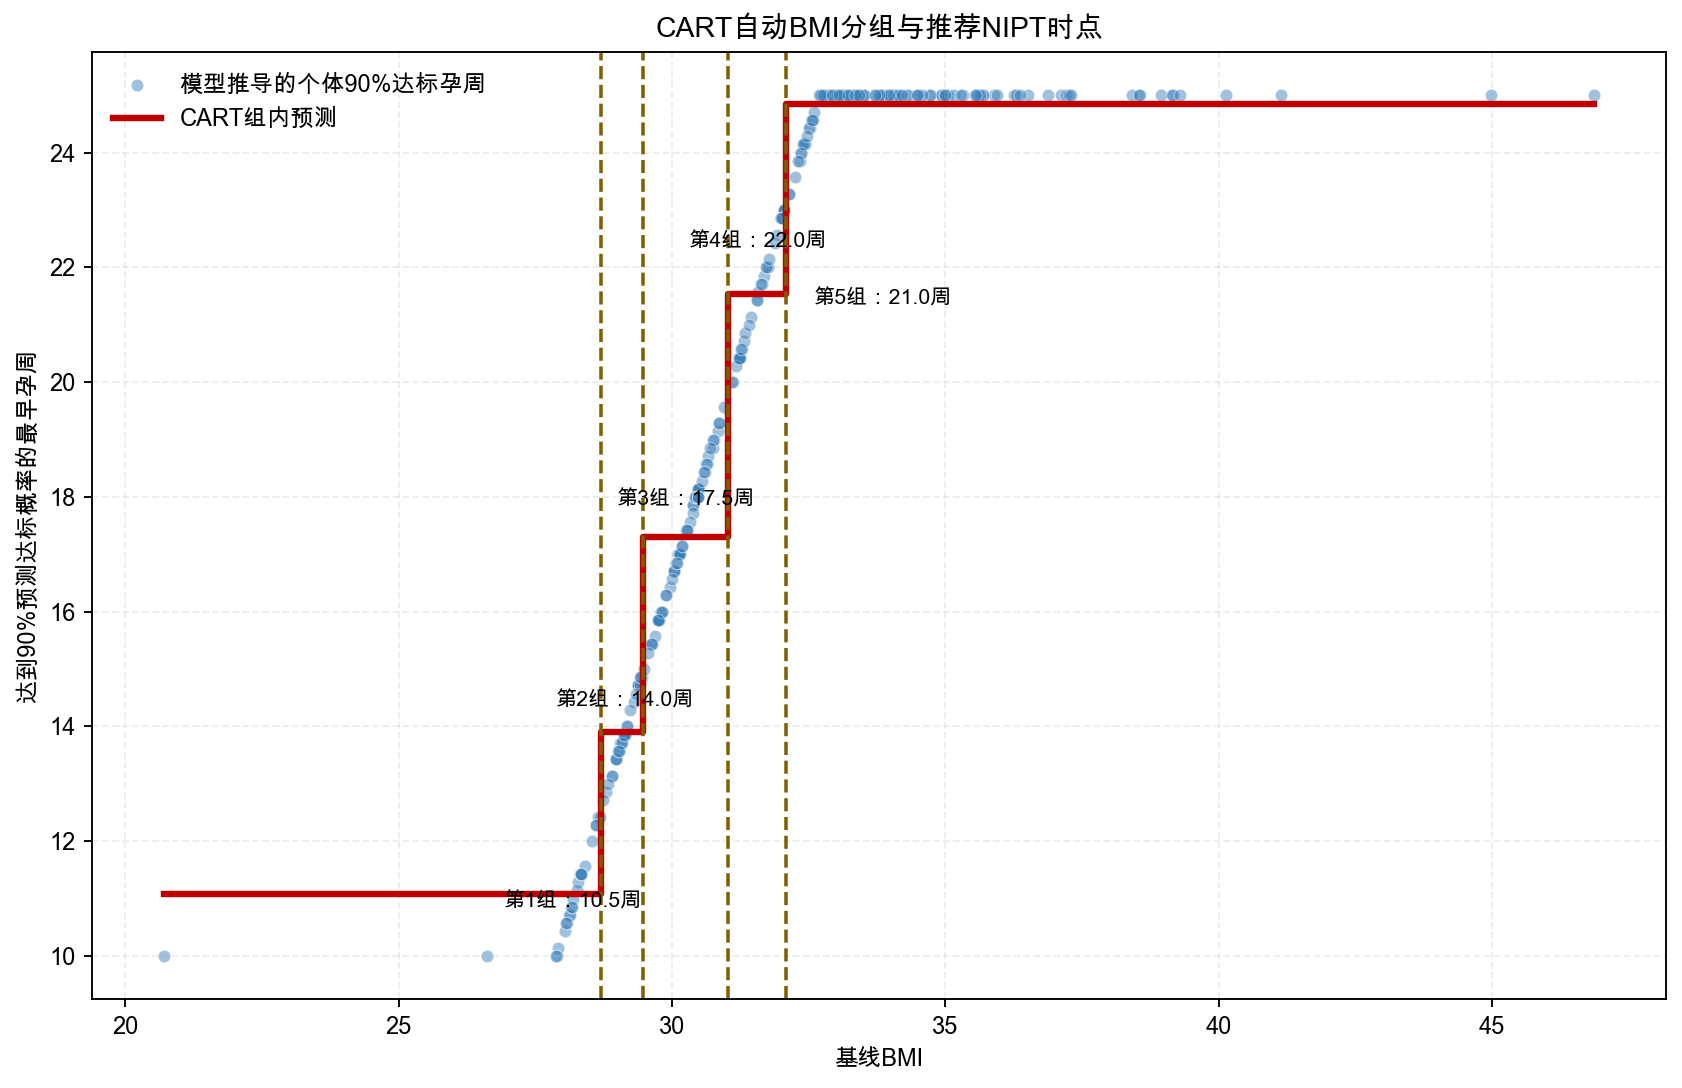
\includegraphics[width=0.96\textwidth]{q2_bmi_groups.png}
  \caption{CART自动BMI分组与推荐NIPT时点}
  \label{fig:q2-cart-groups}
\end{figure}

\begin{table}[H]
  \centering
  \small
  \caption{BMI分组、推荐检测时点及预测可靠性}
  \label{tab:q2-group-result}
  \begin{tabularx}{\textwidth}{c>{\centering\arraybackslash}Xcccc}
    \toprule
    组别 & BMI区间 & 人数 & 推荐孕周 & 平均达标率 & 检测策略 \\
    \midrule
    1 & $B<28.71$ & 25 & 10.5 & 90.1\% & 满足90\%约束 \\
    2 & $28.71\leq B<29.47$ & 31 & 14.0 & 90.1\% & 满足90\%约束 \\
    3 & $29.47\leq B<31.03$ & 67 & 17.5 & 90.1\% & 满足90\%约束 \\
    4 & $31.03\leq B<32.09$ & 35 & 22.0 & 90.2\% & 满足90\%约束 \\
    5 & $B\geq32.09$ & 109 & 21.0 & 85.2\% & 初检后安排复测 \\
    \bottomrule
  \end{tabularx}
\end{table}

由表~\ref{tab:q2-group-result}可知，前四组均选择达到$90\%$平均达标概率的最早时点。第五组在25周内仍无法达到$90\%$，因此按照第~\ref{eq:q2-group-week}式的备用规则，在21.0周达到$85\%$时先进行初检，并对未达标者尽快复测。由此可见，第五组推荐时点早于第四组并非模型认为高BMI孕妇更早达标，而是两组采用了不同的可靠性约束；这种处理体现了对延迟风险的控制。

不同BMI组的达标概率曲线如图~\ref{fig:q2-probability-curves}所示。总体上，BMI越高，同一孕周下的预测达标概率越低，达到$90\%$可靠性所需的时间越晚。最高BMI组在25周内仍未达到$90\%$水平，也说明对其采用“较早初检加复测”比单纯延迟更为合理。

\begin{figure}[H]
  \centering
  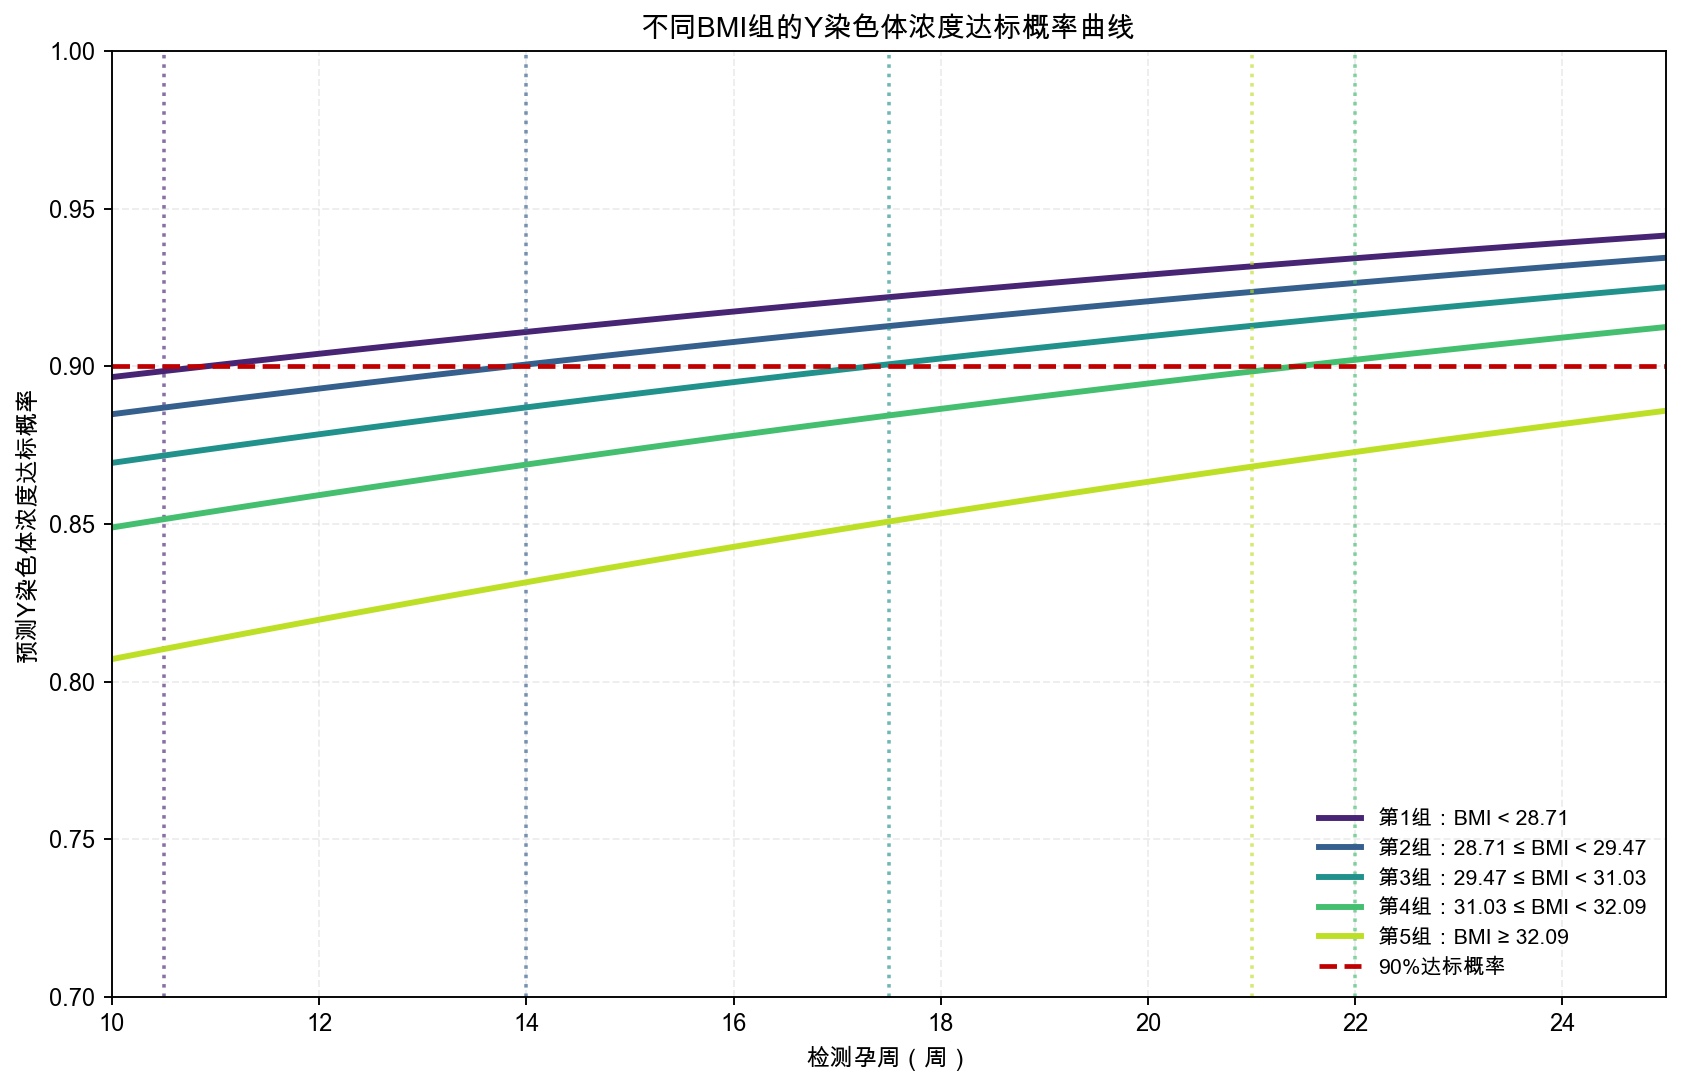
\includegraphics[width=0.96\textwidth]{q2_probability_curves.png}
  \caption{不同BMI组的Y染色体浓度预测达标概率曲线}
  \label{fig:q2-probability-curves}
\end{figure}

\subsection{分组稳定性与检测误差分析}

\subsubsection{BMI切点的Bootstrap稳定性}

对267名孕妇进行300次Bootstrap有放回抽样，每次重新拟合5叶节点CART并记录切点，结果见表~\ref{tab:q2-bootstrap}。

\begin{table}[H]
  \centering
  \caption{300次Bootstrap下BMI切点的稳定性}
  \label{tab:q2-bootstrap}
  \begin{tabular}{cccc}
    \toprule
    切点 & 原始值 & Bootstrap中位数 & 95\%区间 \\
    \midrule
    1 & 28.71 & 28.77 & $[28.48,29.51]$ \\
    2 & 29.47 & 29.53 & $[29.29,30.23]$ \\
    3 & 31.03 & 30.98 & $[30.86,31.07]$ \\
    4 & 32.09 & 32.09 & $[31.95,32.24]$ \\
    \bottomrule
  \end{tabular}
\end{table}

第三、第四切点的区间较窄，稳定性相对较好；第一、第二切点存在一定漂移。由于前两组样本量仅为25和31，表中保留两位小数主要用于模型复现，实际应用时更适合按照约0.5个BMI单位进行近似解释，不宜将切点视为绝对精确的临床边界。

\subsubsection{Y染色体浓度测量误差}

对于19组同次采血重复测序，设两次测量差为$\Delta$。若单次测量误差独立同分布且方差为$\sigma^2$，则

\begin{equation}
  \operatorname{Var}(\Delta)=2\sigma^2.
  \label{eq:q2-error-variance}
\end{equation}

据此估计单次Y染色体浓度测量误差标准差为$\sigma=0.004711$，即0.471个百分点。随后对每条Y染色体浓度加入$N(0,\sigma^2)$扰动，重复200次重新判断$4\%$阈值、拟合概率模型并计算推荐时点。平均有3.26\%的检测记录在扰动后跨越$4\%$阈值。

\begin{table}[H]
  \centering
  \caption{200次测量误差扰动下推荐时点的稳定性}
  \label{tab:q2-error-result}
  \begin{tabular}{cccc}
    \toprule
    组别 & 原始推荐孕周 & 扰动中位数 & 95\%扰动区间 \\
    \midrule
    1 & 10.5 & 12.0 & $[10.0,17.0]$ \\
    2 & 14.0 & 16.0 & $[10.5,20.0]$ \\
    3 & 17.5 & 19.5 & $[16.0,23.5]$ \\
    4 & 22.0 & 22.0 & $[10.0,25.0]$ \\
    5 & 21.0 & 21.5 & $[19.0,25.0]$ \\
    \bottomrule
  \end{tabular}
\end{table}

\begin{figure}[H]
  \centering
  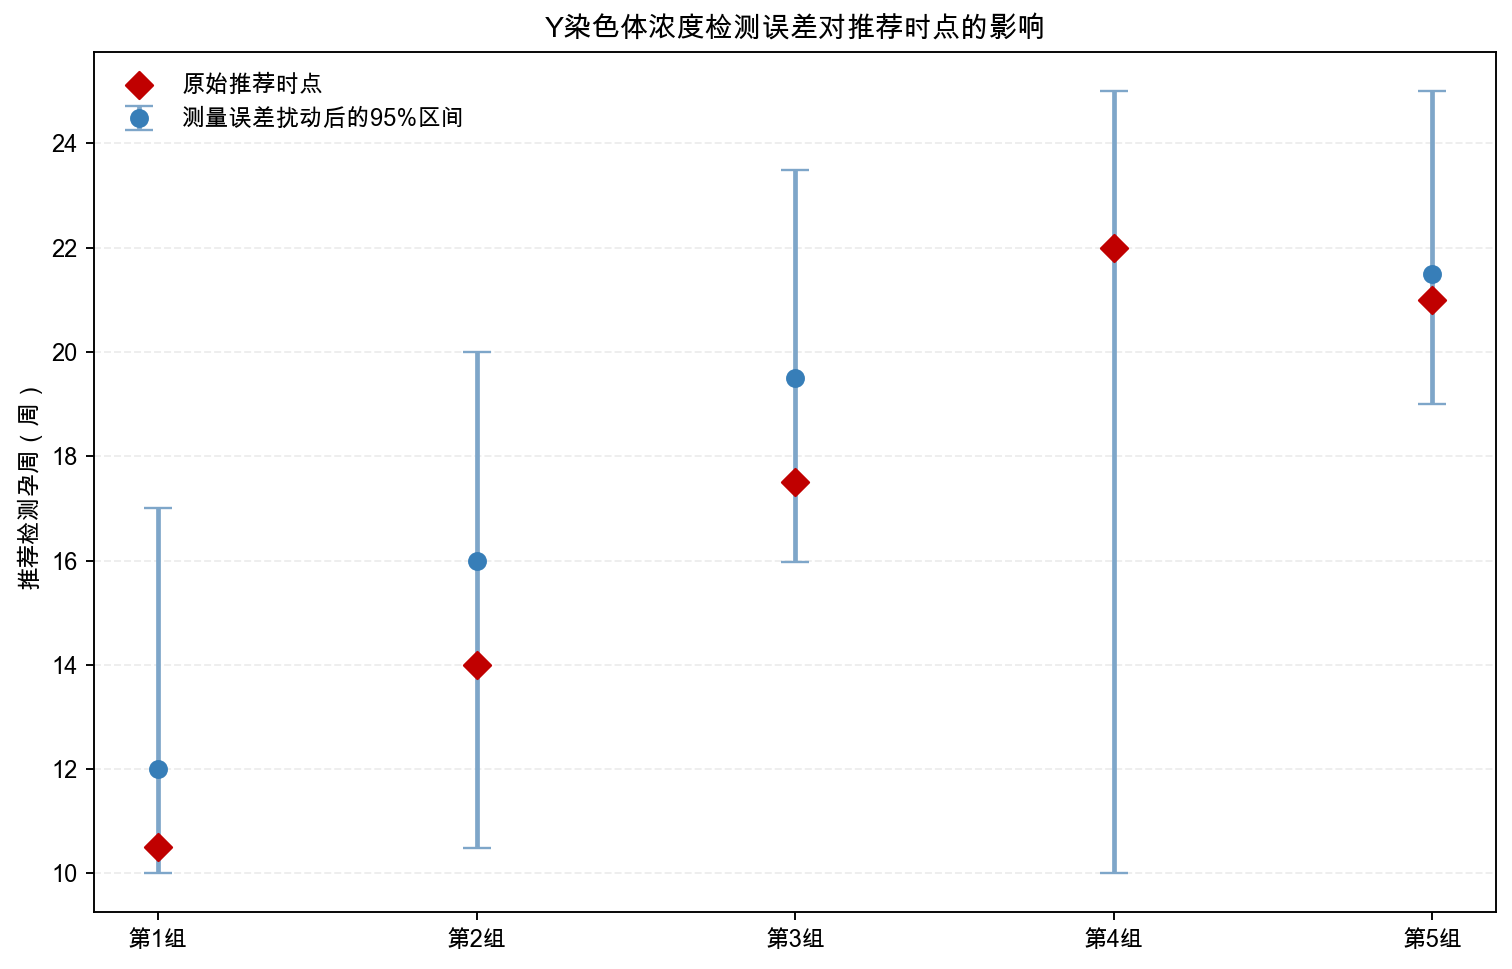
\includegraphics[width=0.90\textwidth]{q2_error_sensitivity.png}
  \caption{Y染色体浓度检测误差对推荐时点的影响}
  \label{fig:q2-error-sensitivity}
\end{figure}

由表~\ref{tab:q2-error-result}和图~\ref{fig:q2-error-sensitivity}可知，第五组推荐时点中位数为21.5周，与原方案方向较为一致；部分中间BMI组的扰动区间较宽，表明接近$4\%$阈值的测量误差可能明显改变推荐时点。因此，表~\ref{tab:q2-group-result}给出的时点应理解为群体层面的基准建议，对于临界BMI或临界Y浓度样本，应结合复测进行个体化判断。

\subsection{问题二结论与模型评价}

本文最终将男胎孕妇划分为$B<28.71$、$[28.71,29.47)$、$[29.47,31.03)$、$[31.03,32.09)$和$B\geq32.09$五组，推荐初次NIPT检测时点依次为10.5、14.0、17.5、22.0和21.0周。其中，最高BMI组由于在25周内不能达到$90\%$预测达标概率，采用21.0周达到$85\%$后先行检测并安排复测的策略。

该方法利用全部纵向检测记录，避免把首次观测达标孕周误认为精确生理达标时间；按孕妇代码分组的交叉验证减少了数据泄漏；一标准误差规则、最小叶节点约束和Bootstrap共同限制模型复杂度；误差扰动进一步量化了$4\%$阈值附近的不确定性。其局限在于样本以高BMI孕妇为主，低BMI组样本量较少，且最终Logistic模型AUC仅为0.5804。因此，本问结果适合作为相似人群的群体检测时点参考，问题三还需加入年龄、身高、体重和测序质量等因素提高个体化能力。

% 问题三由负责同学完成后，将正文写入本文件。
% 建议结构：多因素达标概率模型、BMI分组与时点优化、误差分析。

% 问题四由负责同学完成后，将正文写入本文件。
% 建议结构：标签构造、特征处理、分类模型、分组验证和评价指标。


% ========================= 参考文献 =========================
\bibliographystyle{unsrt}
\bibliography{references}

% =========================== 附录 ===========================
\newpage
\begin{appendices}

\section{支撑材料文件说明}
为避免整段程序挤占论文正文篇幅，源代码、清洗数据和程序结果均作为独立支撑材料随论文一并保存：
\begin{itemize}
  \item 问题二核心程序：\path{code/q2_optimal_timing.py}；
  \item 问题二清洗数据：\path{data/processed/q2_male_cleaned.xlsx}；
  \item 问题二程序结果：\path{results/q2/}；
  \item 问题二正文插图：\path{figures/q2/}。
\end{itemize}
正式提交时，应按照比赛当年的支撑材料要求单独提交程序和数据文件，不在论文正文中粘贴完整代码。

\end{appendices}

\end{document}
